\documentclass{article}
\usepackage{ctex}
\usepackage{graphicx}
\usepackage{amsmath}
\usepackage{geometry}
\usepackage{float}  % 新增，支持 [H] 强制定位
\geometry{a4paper, margin=1in}

\title{\textbf{系统开发工具基础\_实验报告}}
\author{李雨潼 \\ 25020007069}
\date{\today}

\begin{document}

\maketitle

\section*{一、课上实验检查题}

\subsection*{第1题：含空格文件名的批量整理}
\textbf{题目要求：} 创建 input/docs 和 input/tmp；创建 input/docs/notes one.txt（内容为alpha和beta两行）、input/docs/secret.txt（内容为hidden）、input/tmp/empty.txt（空文件）以及 input/run.log（任意两行日志）。显示 q01 的绝对路径，并以长格式列出 input 下全部项目。把 input 下所有 .txt 文件复制到 work/<学号>，保留相对目录结构并正确处理名称中的空格。将复制后的目录权限设为 750，普通文件权限设为 640；生成 inventory.txt，列出相对路径和字节数。

\textbf{执行结果：}
\begin{figure}[H]
    \centering
    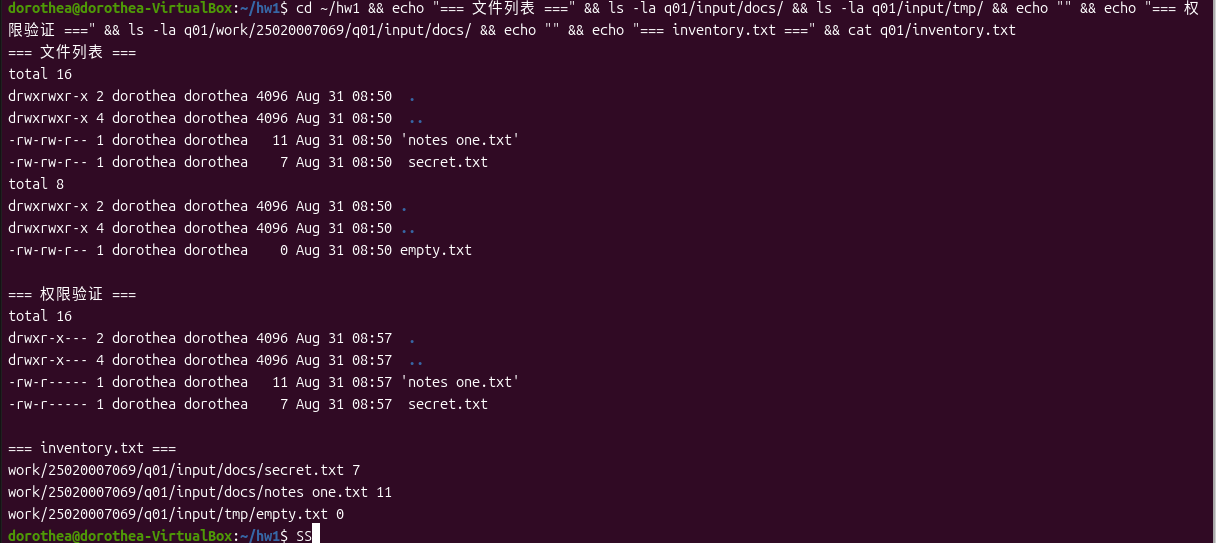
\includegraphics[width=0.9\textwidth]{q1.png}
    \caption{第1题执行结果}
    \label{fig:q1}
\end{figure}

\newpage

\subsection*{第2题：随机访问日志统计}
\textbf{题目要求：} 在 q02 中创建 access.csv，并编写 analyze.sh 脚本，接收 CSV 文件路径。使用 Shell 管道以及 awk、sort、head 等工具，输出 HTTP 5xx 数量最多的前 2 个 path；按次数降序，次数相同时按 path 字典序。输出全部数据的平均 latency_ms，保留两位小数。分别对 access.csv 和一个不存在的文件运行脚本。

\textbf{执行结果：}
\begin{figure}[H]
    \centering
    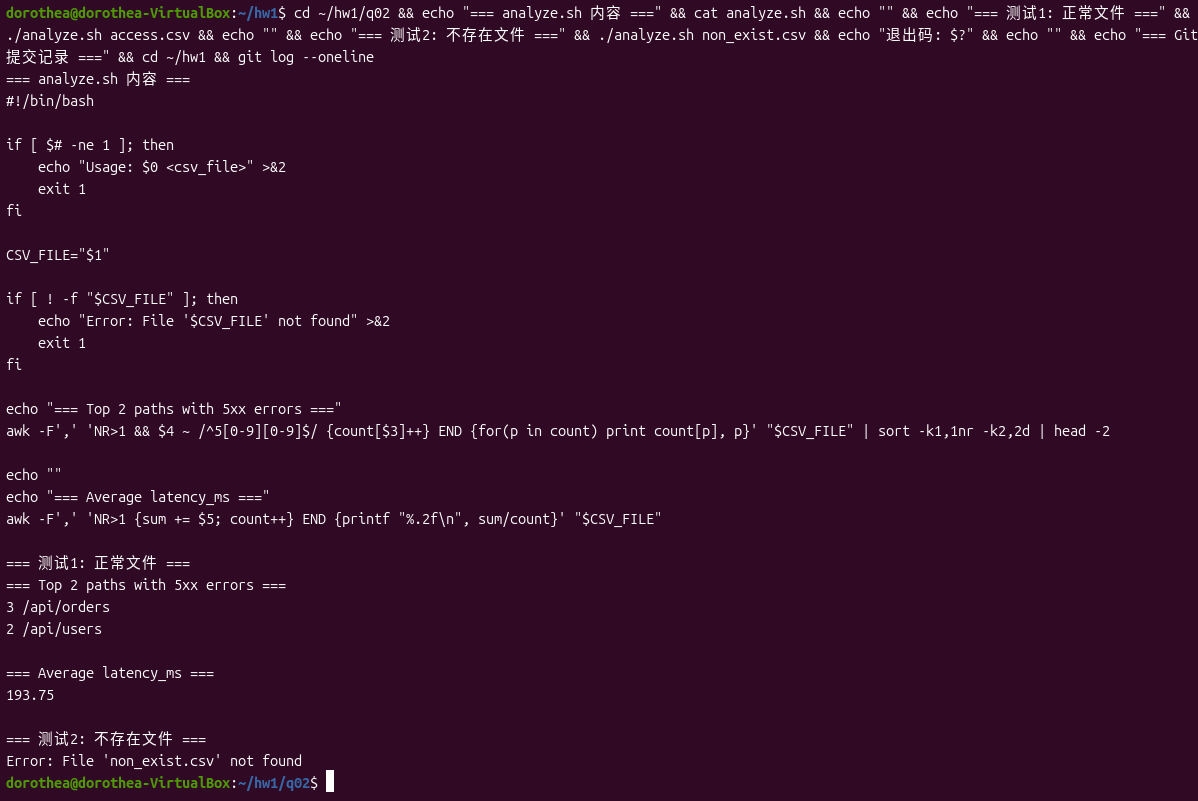
\includegraphics[width=0.9\textwidth]{q2.png}
    \caption{第2题执行结果}
    \label{fig:q2}
\end{figure}

\newpage

\subsection*{第3题：制造、解决并解释一次合并冲突}
\textbf{题目要求：} 在 q03 中从零创建一个 Git 仓库，在 main 创建 config.txt，内容为 mode=normal，并完成初始提交。创建 feature-a，把内容改为 mode=safe 并提交；从初始 main 创建 feature-b，把内容改为 mode=fast 并提交。回到 main，先合并 feature-a，再合并 feature-b；解决冲突时保留 mode=safe，并另加一行 note=reviewed。确认工作区干净，运行 git log --all --graph --decorate --oneline 查看历史。

\textbf{执行结果：}
\begin{figure}[H]
    \centering
    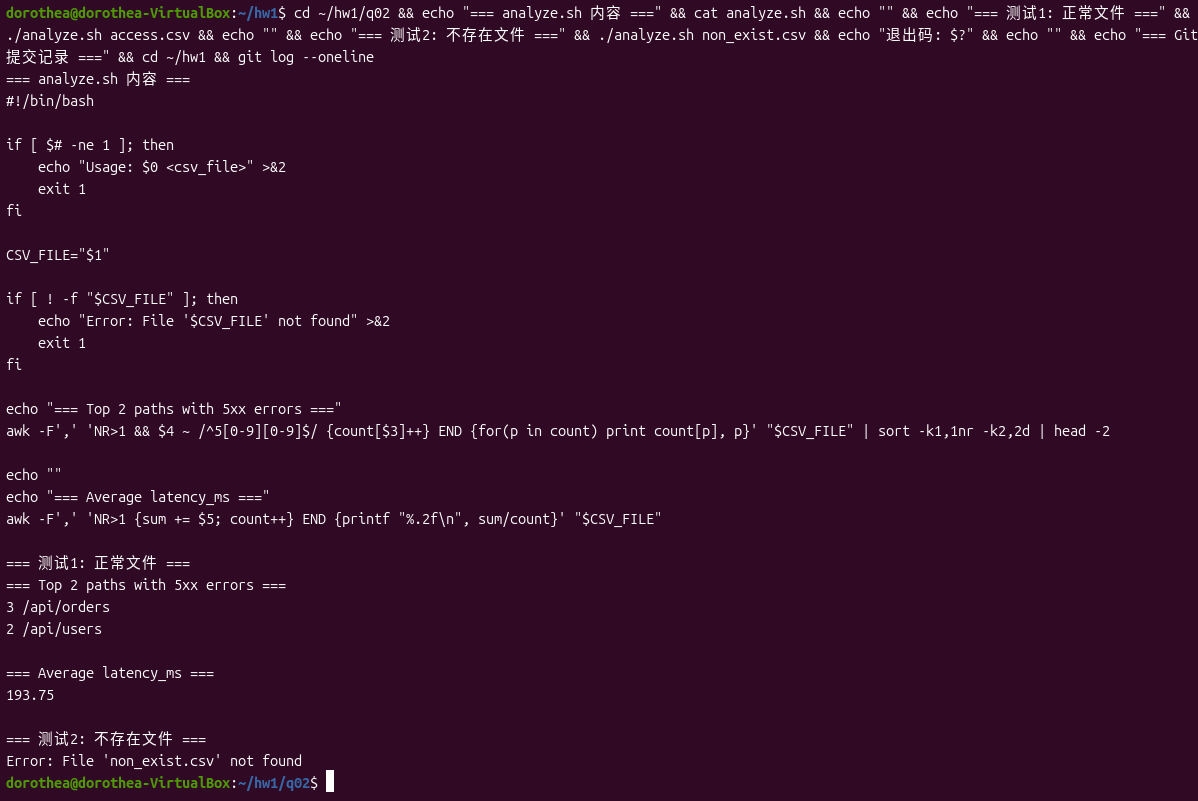
\includegraphics[width=0.9\textwidth]{q3.png}
    \caption{第3题执行结果}
    \label{fig:q3}
\end{figure}

\newpage

\subsection*{第4题：LaTeX文档编辑}
\textbf{题目要求：} 将模板保存为 q04/report.tex，补全内容并从命令行构建 PDF。加入一个带编号和 label 的公式，并在正文中使用 ref 或 eqref 引用。加入一个 2 行 2 列表格，设置 caption 和 label，并在正文中引用该表。使用 latexmk -pdf -halt-on-error 生成 report.pdf。确认 PDF 能打开，且交叉引用不显示 “??”。

\textbf{LaTeX 代码：}
\begin{figure}[H]
    \centering
    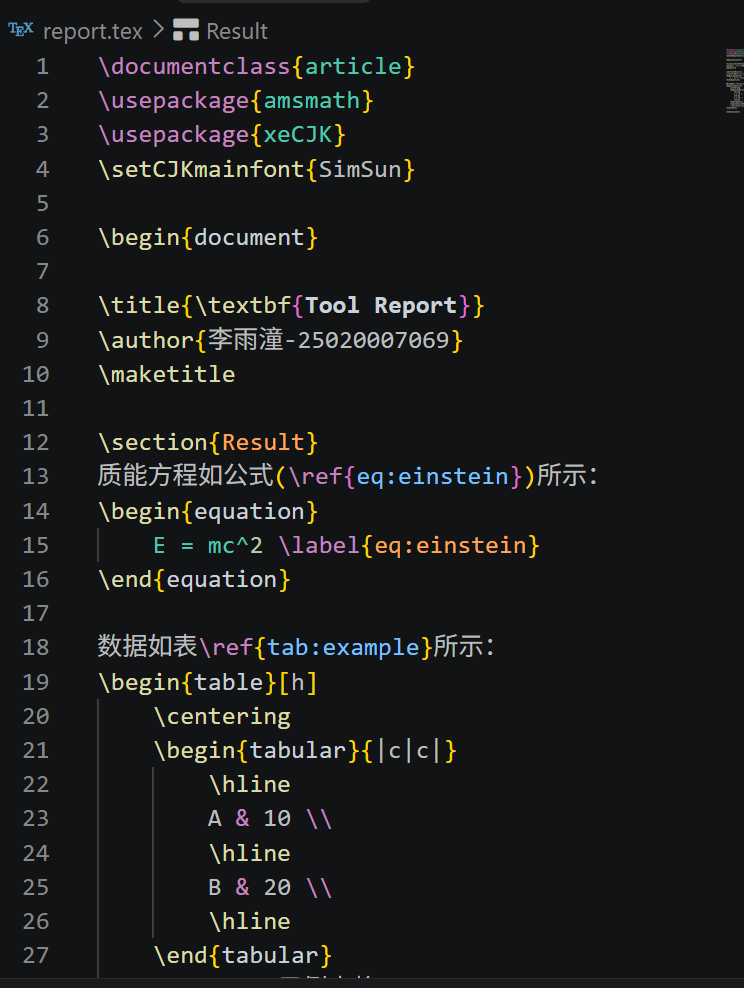
\includegraphics[width=0.9\textwidth]{q4_code1.png}
    \caption{第4题 LaTeX 代码（1）}
    \label{fig:q4_code1}
\end{figure}

\begin{figure}[H]
    \centering
    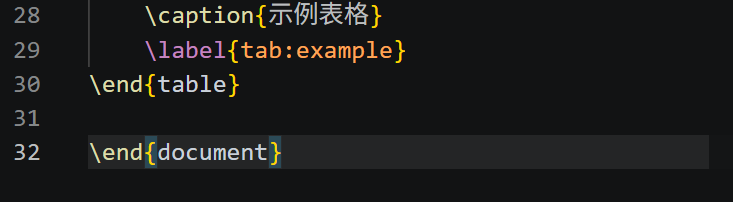
\includegraphics[width=0.9\textwidth]{q4_code2.png}
    \caption{第4题 LaTeX 代码（2）}
    \label{fig:q4_code2}
\end{figure}

\textbf{生成的 PDF：}
\begin{figure}[H]
    \centering
    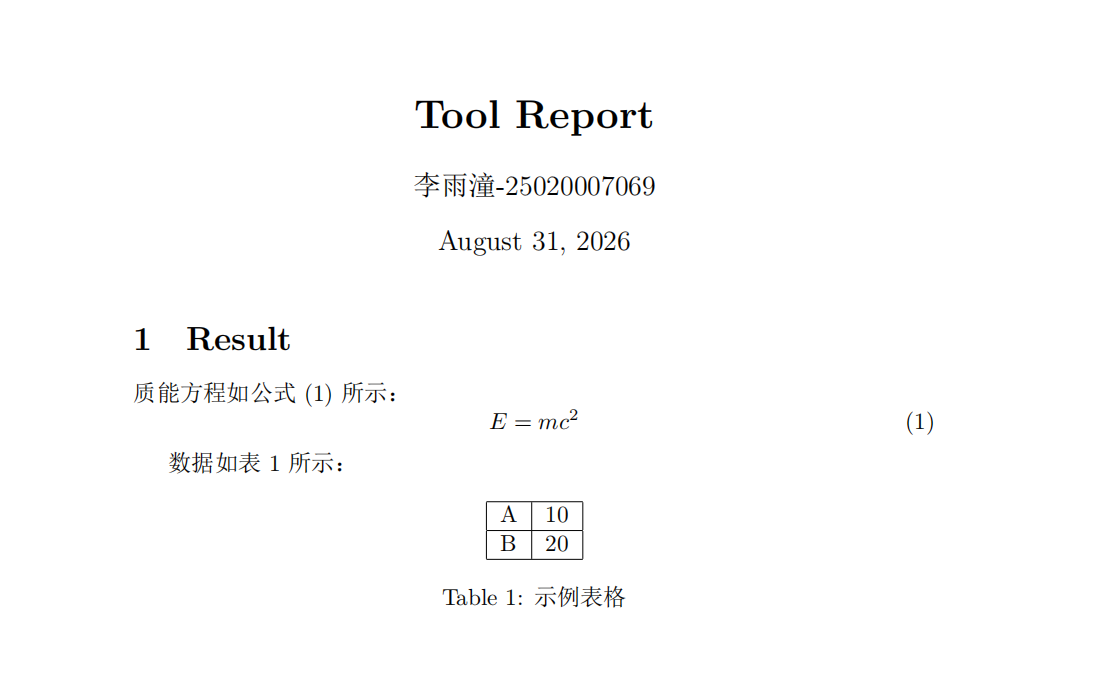
\includegraphics[width=0.7\textwidth]{q4_pdf.png}
    \caption{第4题生成的 PDF}
    \label{fig:q4_pdf}
\end{figure}

\newpage

\section*{二、课后练习（10个实例）}

\subsection*{实例1：ls -l / 分析}
\textbf{题目：} 运行 ls -l /，观察输出，理解每行最前面10个字符的含义。
\begin{figure}[H]
    \centering
    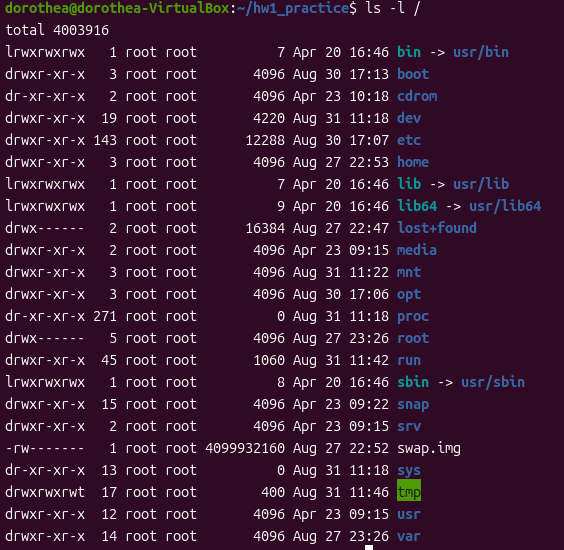
\includegraphics[width=0.9\textwidth]{ex1.png}
    \caption{实例1执行结果}
    \label{fig:ex1}
\end{figure}

\subsection*{实例2：glob 通配符测试}
\textbf{题目：} 新建测试目录，创建一些文件，测试 ls *.txt、ls file?.txt、ls \{a,b,c\}.txt 等模式。
\begin{figure}[H]
    \centering
    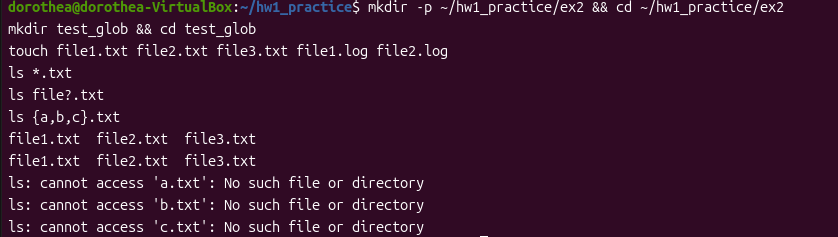
\includegraphics[width=0.9\textwidth]{ex2.png}
    \caption{实例2执行结果}
    \label{fig:ex2}
\end{figure}

\subsection*{实例3：引号区别}
\textbf{题目：} 测试单引号、双引号、反引号的区别，输出含 \$、! 和换行符的字符串。
\begin{figure}[H]
    \centering
    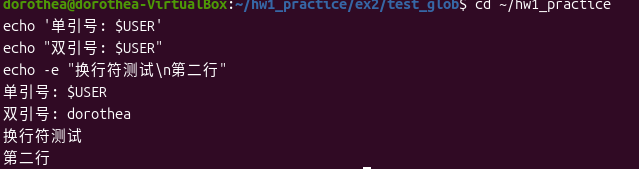
\includegraphics[width=0.9\textwidth]{ex3.png}
    \caption{实例3执行结果}
    \label{fig:ex3}
\end{figure}

\subsection*{实例4：重定向}
\textbf{题目：} 运行 ls /nonexistent /tmp，将 stdout 和 stderr 分别重定向到两个文件，再将两者重定向到同一个文件。
\begin{figure}[H]
    \centering
    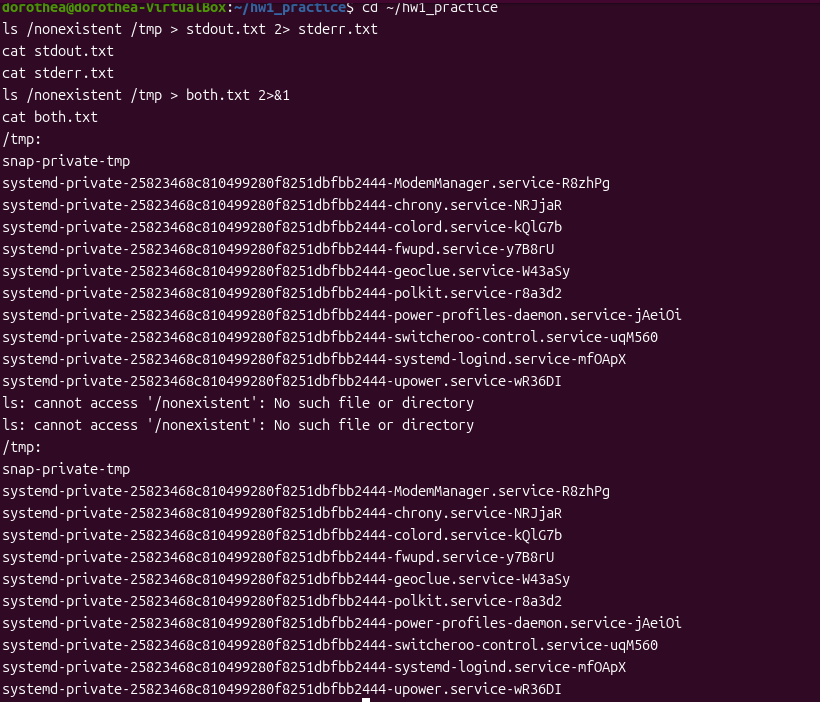
\includegraphics[width=0.9\textwidth]{ex4.png}
    \caption{实例4执行结果}
    \label{fig:ex4}
\end{figure}

\subsection*{实例5：备份文件名}
\textbf{题目：} 写一条命令，把文件复制为带当天日期的备份文件名（例如 notes.txt → notes\_2026-01-12.txt）。
\begin{figure}[H]
    \centering
    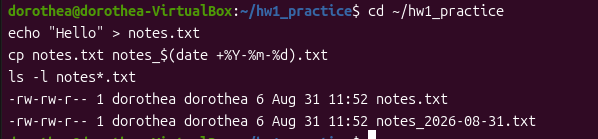
\includegraphics[width=0.9\textwidth]{ex5.png}
    \caption{实例5执行结果}
    \label{fig:ex5}
\end{figure}

\subsection*{实例6：Git 初始提交}
\textbf{题目：} 创建新仓库，创建 recipe.txt，提交初始版本。
\begin{figure}[H]
    \centering
    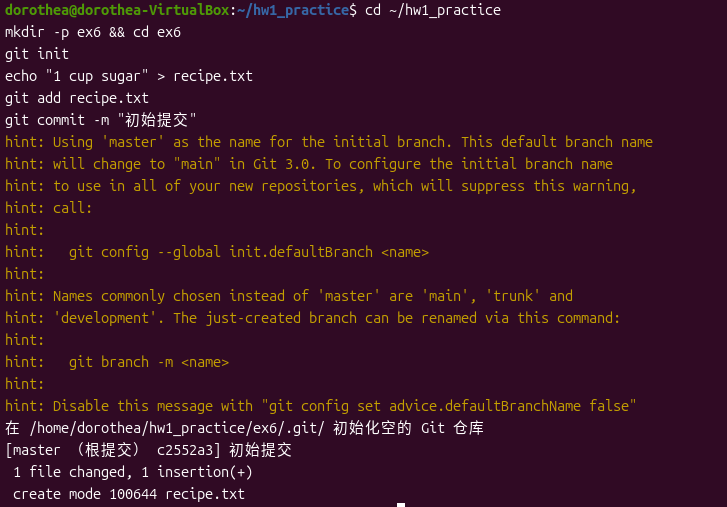
\includegraphics[width=0.9\textwidth]{ex6.png}
    \caption{实例6执行结果}
    \label{fig:ex6}
\end{figure}

\subsection*{实例7：创建分支}
\textbf{题目：} 创建 salty 和 sweet 两个分支，查看所有分支。
\begin{figure}[H]
    \centering
    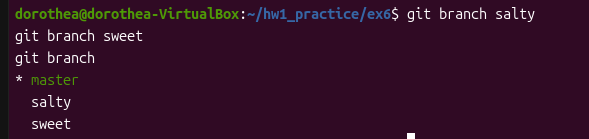
\includegraphics[width=0.9\textwidth]{ex7.png}
    \caption{实例7执行结果}
    \label{fig:ex7}
\end{figure}

\subsection*{实例8：salty 分支修改}
\textbf{题目：} 切换到 salty 分支，修改 recipe.txt 为 "1 cup salt" 并提交。
\begin{figure}[H]
    \centering
    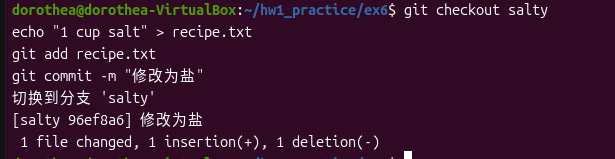
\includegraphics[width=0.9\textwidth]{ex8.png}
    \caption{实例8执行结果}
    \label{fig:ex8}
\end{figure}

\subsection*{实例9：sweet 分支修改}
\textbf{题目：} 切换到 sweet 分支，修改 recipe.txt 为 "2 cups sugar" 并提交。
\begin{figure}[H]
    \centering
    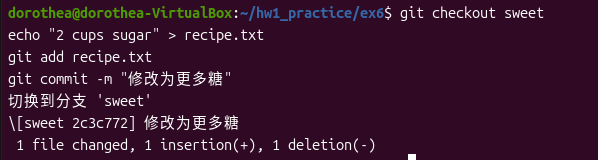
\includegraphics[width=0.9\textwidth]{ex9.png}
    \caption{实例9执行结果}
    \label{fig:ex9}
\end{figure}

\subsection*{实例10：合并冲突}
\textbf{题目：} 切换回 master，先合并 salty，再合并 sweet，观察冲突标记 <<<<<<< HEAD、=======、>>>>>>>。
\begin{figure}[H]
    \centering
    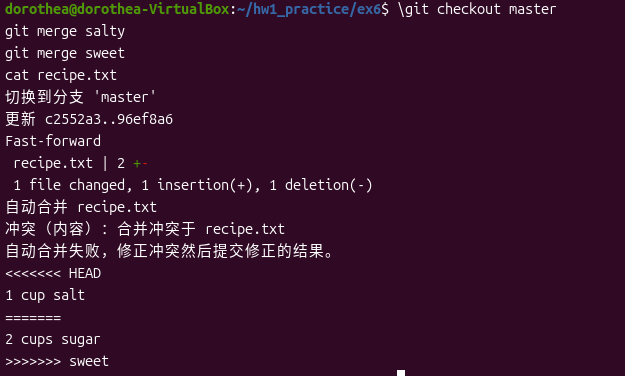
\includegraphics[width=0.9\textwidth]{ex10.png}
    \caption{实例10执行结果}
    \label{fig:ex10}
\end{figure}

\newpage

\section*{三、解题感悟}

通过本次实验，我系统学习了 Shell 基础命令、文件权限管理、文本处理工具（awk、sort、head）、Git 版本控制以及 LaTeX 文档编写。

在 Shell 部分，我掌握了如何正确处理带空格的文件名，以及使用重定向和管道组合命令完成日志统计。在 Git 部分，我亲身体验了分支合并冲突的产生与解决过程，理解了冲突标记的含义，并学会了使用 git log --graph 查看分支历史。在 LaTeX 部分，我学会了编写带交叉引用的公式和表格文档，并成功生成了 PDF。

此外，课后10个实例让我进一步巩固了 glob 通配符、引号区别、重定向、备份脚本等实用技能。所有代码均已提交至 GitHub，形成了完整的 commit 记录。

这次实践让我深刻体会到，命令行工具和版本控制是软件开发中不可或缺的基础技能，未来我会继续加强这方面的练习。

\end{document}